\Hefteintrag{1.2}{Übersicht Befehlsarten}{
\label{sec:befehlsarten}

Es gibt viele verschiedene Befehlsarten. Die für uns wichtigsten sind:

\begin{tabularx}{\textwidth}{b{0.5cm}>{\centering\arraybackslash}b{3.5cm}>{\centering\arraybackslash}b{3.5cm}>{\centering\arraybackslash}X>{\centering\arraybackslash}X}
\emphColA{Art}
& \emphColA{Online-Karol} 
& \emphColA{Blockly} 
& \emphColA{Java} 
& \emphColA{Struktogramm} \\ 

%\rotatebox{90}{\Loesung{einf. Befehl\color{black}}{\lineheight}}

\LoesungLeer{\multicolumn{5}{l}{\color{blue} einf. Befehl\color{black}}\\}
%

&
\includegraphics[width=\linewidth]{_Aufgaben//BlocklyJava_Skript//img/H02_karol_command.png}
&
\includegraphics[width=\linewidth]{_Aufgaben//BlocklyJava_Skript//img/H02_blockly_command.png}
&\LoesungKaro{karol.linksDrehen(1);\newline System.out.println("abc");}{4}
&\LoesungKaro{}{4}\\

\Loesung{\multicolumn{5}{l}{\color{blue} Verzweigung\color{black}}\\}

%\rotatebox{90}{\LoesungLine{Verzweigung}{1}}
&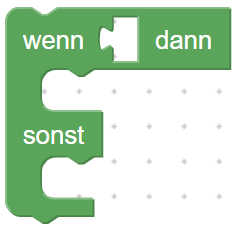
\includegraphics[width=\linewidth]{_Aufgaben//BlocklyJava_Skript//img/H02_karol_if-else.png}
&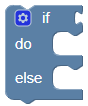
\includegraphics[width=2.5cm]{_Aufgaben//BlocklyJava_Skript//img/H02_blockly_if-else.png}
&\LoesungKaro{if(<Bedingung>) \{ \newline \indent\hspace{1cm} // wenn \newline \} else \{ \newline \indent\hspace{1cm} // sonst \newline \}}{7}
&\LoesungKaro{}{7}\\


\Loesung{\\\multicolumn{5}{l}{\color{blue} Schleife / bedingte Wiederholung\color{black}}\\}

%\rotatebox{90}{\LoesungLine{Schleife}{1}}
&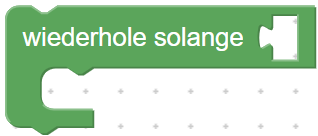
\includegraphics[width=\linewidth]{_Aufgaben//BlocklyJava_Skript//img/H02_karol_while.png}
&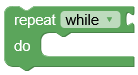
\includegraphics[width=\linewidth]{_Aufgaben//BlocklyJava_Skript//img/H02_blockly_while.png}
&\LoesungKaro{while(<Bedingung>) \{\newline...\newline\}}{5}
&\LoesungKaro{}{5}\\

\Loesung{\multicolumn{5}{l}{\color{blue} Zählschleife\color{black}}\\}

%\rotatebox{90}{\LoesungLine{Zählschleife}{1}}
&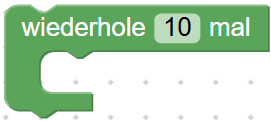
\includegraphics[width=\linewidth]{_Aufgaben//BlocklyJava_Skript//img/H02_karol_for.png}
&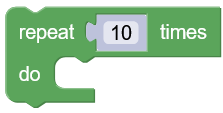
\includegraphics[width=\linewidth]{_Aufgaben//BlocklyJava_Skript//img/H02_blockly_for.png}
&\LoesungKaro{for(int i=0; i<10; i++) \{\newline...\newline\}}{7}
&\LoesungKaro{}{7}\\

\Loesung{\multicolumn{5}{l}{\color{blue} Methodendeklaration\color{black}}\\}

%\rotatebox{90}{\LoesungLine{M-Deklaration}{1}}
&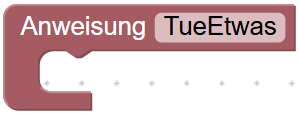
\includegraphics[width=\linewidth]{_Aufgaben//BlocklyJava_Skript//img/H02_karol_funcdef.png}
&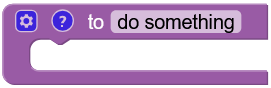
\includegraphics[width=\linewidth]{_Aufgaben//BlocklyJava_Skript//img/H02_blockly_funcdef.png}
&\LoesungKaro{public void doSomething() \{\newline...\newline\}}{5}
&\LoesungKaro{}{5}\\

\Loesung{\multicolumn{5}{l}{\color{blue} Methodenaufruf\color{black}}\\}

%\rotatebox{90}{\LoesungLine{M-Aufruf}{1}}
&
\includegraphics[width=\linewidth]{_Aufgaben//BlocklyJava_Skript//img/H02_karol_funccall.png}
&
\includegraphics[width=\linewidth]{_Aufgaben//BlocklyJava_Skript//img/H02_blockly_funccall.png}
&\LoesungKaro{doSomething();}{2}
&\LoesungKaro{}{2}\\

\Loesung{\\\multicolumn{5}{l}{\color{blue} Kommentar\color{black}}\\}

%\rotatebox{90}{\LoesungLine{Kommentar}{1}}
&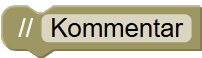
\includegraphics[width=\linewidth]{_Aufgaben//BlocklyJava_Skript//img/H02_karol_kommentar.png}
&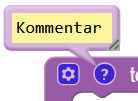
\includegraphics[width=0.8\linewidth]{_Aufgaben//BlocklyJava_Skript//img/H02_blockly_kommentar.png}
&\LoesungKaro{// Kommentar}{3}
&\LoesungKaro{}{3}\\


\Loesung{\\\multicolumn{5}{l}{\color{blue} Konstruktor\color{black}}\\}

%\rotatebox{90}{\LoesungLine{Konstruktor}{1}}
&%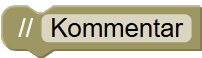
\includegraphics[width=\linewidth]{_Aufgaben//BlocklyJava_Skript//img/H02_karol_kommentar.png}
&
\includegraphics[width=1.1\linewidth]{_Aufgaben//BlocklyJava_Skript//img/H02_blockly_ctrdef.png}
&\LoesungKaro{public MeineKlasse() \{\newline...\newline\}}{4}
&\LoesungKaro{}{4}\\


\Loesung{\multicolumn{5}{l}{\color{blue} Objekt erstellen\color{black}}\\}

%\rotatebox{90}{\LoesungLine{Objekt erstellen}{1}}
%&%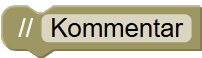
\includegraphics[width=\linewidth]{_Aufgaben//BlocklyJava_Skript//img/H02_karol_kommentar.png}
&
&
\includegraphics[width=1.1\linewidth]{_Aufgaben//BlocklyJava_Skript//img/H02_blockly_ctrcall.png}
&\LoesungKaro{new MeineKlasse();}{2}
&\LoesungKaro{}{2}\\

\end{tabularx}

}